\documentclass[12pt]{article}

%-------------PACKAGES------------- 
\usepackage[margin=1in]{geometry} 
\usepackage{amsmath,amsthm,amssymb}
\usepackage{pgfplots}
\usepackage{float}
\usepackage{braket}
\usepackage{titling}
\usepackage{wrapfig}
\usepackage{tikz}
\usepackage{mwe}
\usepackage{enumitem}
\usepackage{mathtools}
\usepackage{scrextend}
\usepackage{listings}
\usepackage{color}
\usepackage{caption}
\usepackage{subcaption}
\usepackage{algorithm,algpseudocode}
\usetikzlibrary{shapes,arrows,chains}
\usetikzlibrary[calc]

%-------------FORMATTING-------------
\setlength{\droptitle}{-7.5em} 
\setlength{\parindent}{0pt}
\def\LW{\dimexpr.25\linewidth-.5em} 
\tikzstyle{line} = [draw, -latex']

%--------------COMMANDS--------------
\newcommand{\N}{\mathbb{N}}
\newcommand{\Z}{\mathbb{Z}}
\newcommand{\R}{\mathbb{R}}
\newcommand{\C}{\mathbb{C}}
%\renewcommand{\qedsymbol}{\filledbox}

\DeclarePairedDelimiter \abs{\lvert}{\rvert}%
\DeclarePairedDelimiter \babs{\bigg\lvert}{\bigg\rvert}%
\DeclarePairedDelimiter \norm{\lVert}{\rVert}%

%------------ENVIRONMENTS------------- 
\newenvironment{theorem}[2][]{\begin{trivlist}
		\item[{\bfseries #1}\hskip \labelsep {\bfseries #2.}]}{\end{trivlist}}
\newenvironment{lemma}[2][Lemma]{\begin{trivlist}
		\item[\hskip \labelsep {\bfseries #1}\hskip \labelsep {\bfseries #2.}]}{\end{trivlist}}
\newenvironment{exercise}[2][Exercise]{\begin{trivlist}
		\item[\hskip \labelsep {\bfseries #1}\hskip \labelsep {\bfseries #2.}]}{\end{trivlist}}
\newenvironment{reflection}[2][Reflection]{\begin{trivlist}
		\item[\hskip \labelsep {\bfseries #1}\hskip \labelsep {\bfseries #2.}]}{\end{trivlist}}
\newenvironment{proposition}[2][Proposition]{\begin{trivlist}
		\item[\hskip \labelsep {\bfseries #1}\hskip \labelsep {\bfseries #2.}]}{\end{trivlist}}
\newenvironment{corollary}[2][Corollary]{\begin{trivlist}
		\item[\hskip \labelsep {\bfseries #1}\hskip \labelsep {\bfseries #2.}]}{\end{trivlist}}
\newenvironment{definition}[2][]{\begin{trivlist}
		\item[{\bfseries #1}\hskip \labelsep {\bfseries #2.}]}{\end{trivlist}}
\theoremstyle{remark}
\newtheorem*{remark}{Remark}

%-------------CODE-STYLE------------
\definecolor{dkgreen}{rgb}{0,0.6,0}
\definecolor{gray}{rgb}{0.5,0.5,0.5}
\definecolor{mauve}{rgb}{0.58,0,0.82}
\lstset{frame=tb,
	language=C++,
	aboveskip=3mm,
	belowskip=3mm,
	showstringspaces=false,
	columns=flexible,
	basicstyle={\small\ttfamily},
	numbers=none,
	numberstyle=\tiny\color{gray},
	keywordstyle=\color{blue},
	commentstyle=\color{dkgreen},
	stringstyle=\color{mauve},
	breaklines=true,
	breakatwhitespace=true,
	tabsize=3
}

\tikzset{
	path image/.style={
		path picture={
			\node at (path picture bounding box.center) {
				\includegraphics[height=3cm]{example-image}};}},
	path tikzimage/.style={
		path picture={
			\node at (path picture bounding box.center)
			[circle, fill=blue!50, scale=2, text=yellow]{Bravo};}}
}

\lstset{
	morekeywords={end}
}

%------------------------------------ 
%---------START-OF-DOCUMENT----------
%------------------------------------
\begin{document}
	
	\title{Paper Summary}
	\author{David Miller \\ 
		CIS 5930: Social Network Mining} 
	
	\maketitle 
	
	Current recommender systems provide accurate recommendations to static data, that is temporal dynamics are inferred after they are observed. The Recurrent Recommender Network (RRN) is able to predict future behavior trajectories. The model computes update functions
	\begin{align*}
		\hat{r}_{ij | t} = f(u_{it}, m_{jt}) \text{ and } & u_{i,t+1} = g(u_{it}, \{r_{ij | t}\}) \\
		& m_{j,t+1} = h(m_{jt},\{r_{ij | t}\})
	\end{align*}
	where $\hat{r}_{ij|t}$ denotes the predicted rating for user $i$ on movie $j$, $r_{ij|t}$ is the actual rating, at time step $t$, and $u_i$ and $m_j$ be latent attributes for user $i$ and movie $j$. The functions $f$, $g$ and $h$ are learned such that we can infer a new user’s state directly without need for further optimization \cite{paper}. The way the RNN algorithm determines these functions is through four steps:
	\begin{enumerate}
		 \item Movie and user states that have ratings $k_1, \dots, k_N$ for movies $m_1, \dots, m_N$ and 0 otherwise (user is either new or has not seen the movie) for each time value $t$  
		 \item Compute stationary rating components, such as long term preferences or liked genres, and incorporate them with profile vectors $u_i$ and $m_j$ from step 1
		 \item Take the latest observations and update states and make predictions based on the newly updated states. 
		 \item Find optimal parameters that yield predictions that are close to actual ratings via
		 $$ \min\limits_{\theta} \sum\limits_{(i,j,t) \in I_{train}} \big( r_{ij|t} - \hat{r}_{ij|t}(\theta) \big)^2 + R(\theta) $$
		 where $\theta$ are all the parameters to be learned, $I_{learned}$ is the set of observed , and $R$ denotes some regularization function \cite{paper}.
	\end{enumerate}
	
	\begin{wrapfigure}{r}{0.4\textwidth}
		\vspace{-15pt}
		\hspace{-1pt}
		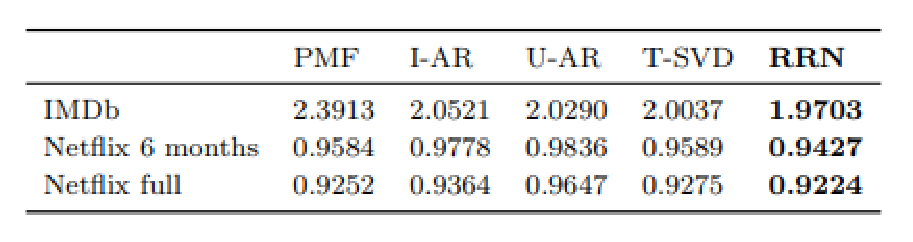
\includegraphics[height=2cm,width=0.45\textwidth]{fig3.eps}
	\end{wrapfigure}
	
	In terms of results, RNN outperforms other models with respect to root mean square error (RMSE). In figure 1 , RNN only used 20-dimensional stationary factors and 40-dimensional embedding factors whereas PMF and TimeSVD++ use dimensionality 160 and AutoRec used 500-dimensional embeddings. In terms of future work, I think this algorithm should be commercialized due to its accuracy with low dimensionality compared to current recommender systems in place. Another future direction they can take is to locally mount this "light-weight" algorithm on peoples computer to reduce power consumption of the company. It seems as if the algorithm may be efficient enough to be run on persoanl computers without causing any slowdowns. 
	
	\newpage
	
	Three strengths I found with the paper are
	\begin{enumerate}
		\item The accuracy RNN achieves with such low dimensionality.
		\item While being sparse (90 times sparser than other methods), it does not suffer from this fact. This is due to the model learning the functions rather than the parameters.
		\item RNN still provides accurate results for users with very few ratings.
	\end{enumerate} 
	\vspace{0.5cm}
	
	Three weaknesses I found with the paper are
	\begin{enumerate}
		\item RNN relies on datasets that are private to Netflix, IMDb, etc. 
		\item Although accurate, users with few ratings produces noisy predictions.
		\item Although smaller time steps allow for frequent updates and the ability to capture short term effects, it increase the time complexity (and inaccuracy) by increasing FLOPS.
	\end{enumerate}
	\vspace{0.5cm}
	
	Questions for the reader
	\begin{enumerate}
		\item What is the time complexity of RNN?
		\item The authors are from Google, LinkedIn, UT Austin and Carnegie Melon. I assume Google will take most, if not all, of the copyrights for the algorithm but who "owns" this algorithm?
		\item Need some clarity with Rating Emissions. Ask presenter about this.
	\end{enumerate}
	\vspace{0.5cm}
	
	\begin{thebibliography}{unsrt}
		\bibitem{paper}
		Chao-Yuan Wu, Amr Ahmed, Alex Beutel, Alexander J. Smola, How Jing \emph{Recurrent Recommender Networks}, KDD’17, August 13-17, 2017, Halifax, NS, Canada.
	\end{thebibliography}
	
\end{document}\documentclass[12pt]{article}